\section{Experiments}

% \begin{table}[t]
% \caption{Performance on TSRBench accuracy (\%) across reasoning tasks compared with various agentic frameworks. The best results are highlighted in \textbf{bold}. All methods use GPT-5-nano as the base model. }
% \label{tab:tsrbench_nano_main}
% \centering
% \resizebox{1.0\columnwidth}{!}{%
% \begin{tabular}{lccccc}
% \toprule
% Method & Overall & Perception & Reasoning & Prediction & Decision \\ 
% \midrule
% CoT          & 40.05 & 48.57 & 36.84 & 46.30 & 28.57 \\
% ReAct               & 40.78 & 55.71 & 36.26 & 43.52 & 31.75 \\
% Self-Reflection     & 40.29 & 50.00 & 40.93 & 38.89 & 30.16 \\
% Multi-Reflection  & 42.96 & 62.85 & 33.92 & 54.63 & 25.40 \\
% TSci                & 40.53 & 65.71 & 33.33 & 43.52 & 26.98 \\
% \midrule
% TimeClaw (Ours)    & \textbf{49.76} & \textbf{64.29} & \textbf{43.86} & \textbf{59.26} & \textbf{33.33} \\
% % TimeClaw ($k=3$)    & 48.06 & 61.43 & \textbf{45.61} & 52.78 & 31.75 \\
% \bottomrule
% \end{tabular}%
% }
% \end{table}
\renewcommand{\arraystretch}{1.2}
\begin{table*}[t]
\caption{Performance on TSRBench across open-ended temporal reasoning tasks. The best and second-best results in each metric column are highlighted in \textbf{bold} and \underline{underlined}, respectively. All methods use GPT-5-nano as the base model. \method achieves the best average accuracy while using the fewest tokens.}
\label{tab:tsrbench_nano_main}
\centering
\resizebox{\textwidth}{!}{%
\begin{tabular}{lcccccc}
\toprule
Method & Perception & Reasoning & Prediction & Decision Making & Avg. Accuracy (\%) & Avg. Token Consumption \\ 
\midrule
CoT \cite{wei2022chain} & 48.57 & 36.84 & 46.30 & 28.57 & 40.05 & 22,274 \\
ReAct \cite{DBLP:conf/iclr/YaoZYDSN023} & 55.71 & 36.26 & 43.52 & \underline{31.75} & 40.78 & 25,165 \\
Self-Reflection \cite{DBLP:journals/corr/abs-2405-06682} & 50.00 & \underline{40.93} & 38.89 & 30.16 & 40.29 & 25,799 \\
Multi-Agent Reflection \cite{DBLP:conf/icml/YuanX25} & 62.85 & 33.92 & \underline{54.63} & 25.40 & \underline{42.96} & 45,279 \\
TSci \cite{DBLP:journals/corr/abs-2510-01538} & \textbf{65.71} & 33.33 & 43.52 & 26.98 & 40.53 & 51,273 \\
% TS-Agent \cite{DBLP:journals/corr/abs-2510-01538} & \underline{64.29} & 33.33 & 43.52 & 26.98 & 43.7 & 98,058 \\
\midrule
\method (Ours)    & \underline{64.29} & \textbf{43.86} & \textbf{59.26} & \textbf{33.33} & \textbf{49.76} & \textbf{15,979} \\
% TimeClaw ($k=3$)    & 61.43 & \textbf{45.61} & 52.78 & 31.75 & 48.06 & -- \\
\bottomrule
\end{tabular}%
}
\end{table*}
\renewcommand{\arraystretch}{1.0}


We comprehensively evaluate \method on three recent benchmarks spanning diverse application domains, demonstrating its effectiveness across a wide range of open-ended contextualized time-series scenarios.


\noindent\textbf{Benchmarks and Evaluation Focus.}
We evaluate \method on three complementary benchmarks. Context-is-Key (CiK) \citep{DBLP:conf/icml/WilliamsAMZSRRL25} examines context utilization in context-aware time-series reasoning; TSRBench \citep{DBLP:journals/corr/abs-2601-18744} evaluates open-ended generalist capability through multi-task multimodal scenarios; and TSAIA \citep{DBLP:journals/corr/abs-2509-01822} focuses on practical domain-specific financial analysis. We provide details in Appendix \ref{ap:dataset_details}


\noindent\textbf{Baselines.}
We compare \method with a broad set of baselines spanning five families. 
(a) \textit{Traditional time-series models}, including statistical forecasting methods ARIMA and ETS \citep{shchur2023autogluon}, as well as neural forecasting models DLinear \citep{DBLP:conf/aaai/ZengCZ023} and PatchTST \citep{DBLP:conf/iclr/NieNSK23}. 
(b) \textit{Time-series foundation models}, including Chronos-family models \citep{DBLP:journals/tmlr/AnsariSTZMSSRPK24, DBLP:journals/corr/abs-2510-15821}, Lag-Llama \citep{rasul2023lag}, and Moirai-family models \citep{DBLP:conf/icml/WooLKXSS24}. 
(c) \textit{LLMs and agents designed for time series}, including UniTime \citep{DBLP:conf/www/LiuHLDLHZ24}, Time-LLM \citep{DBLP:conf/iclr/0005WMCZSCLLPW24}, TS-Agent \citep{DBLP:journals/corr/abs-2510-07432}, and TSci \citep{DBLP:journals/corr/abs-2510-01538}.
(d) \textit{Open-source LLMs}, such as LLaMA3-70B \citep{DBLP:journals/corr/abs-2407-21783}.
(e) \textit{General agentic pipelines}, including direct prompting, chain-of-thought prompting \citep{DBLP:conf/nips/Wei0SBIXCLZ22}, ReAct \citep{DBLP:conf/iclr/YaoZYDSN023}, self-reflection \citep{DBLP:journals/corr/abs-2405-06682}, and multi-agent reflection \citep{DBLP:conf/icml/YuanX25}. 
Additional details are provided in Appendix~\ref{ap:baselines}.




\begin{figure}[t]
\centering
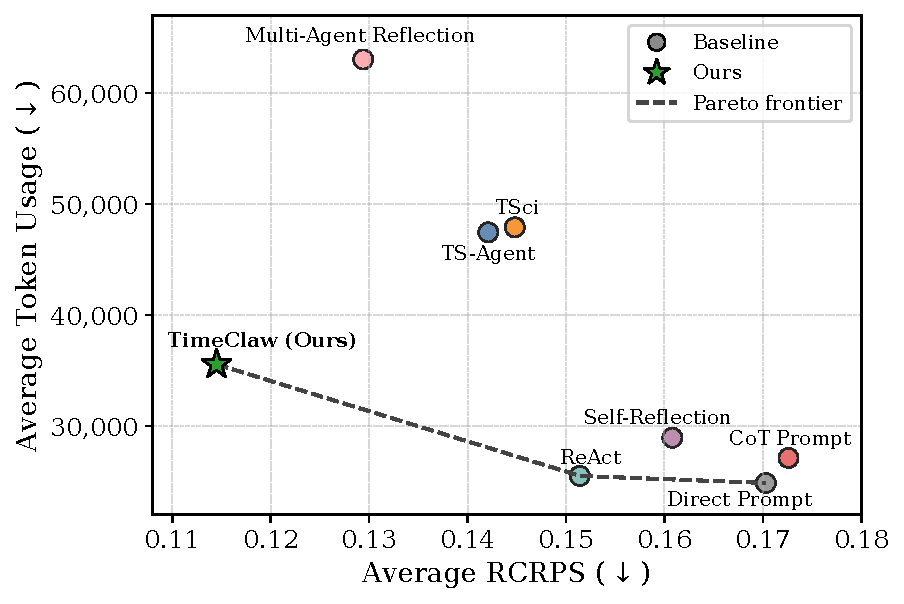
\includegraphics[width=\linewidth]{figures/hyperparameter/cik_rcrps_vs_token.pdf}
\caption{Performance-efficiency trade-off on CiK. Among methods with reported token usage, \method achieves the best RCRPS with substantially lower token consumption than the strongest multi-agent baseline.}
\label{fig: teasing}
\end{figure}


\subsection{Context Matters for Time Series, and \method Uses It More Effectively}

\noindent\textbf{Metrics.}
RCRPS is the primary metric of CiK. It emphasizes context-relevant regions and penalizes violations of task-specific constraints. We additionally report sMAPE as a widely used metric in time series. We also report token usage when applicable. Detailed metric definitions are provided in Appendix~\ref{ap:metrics}.

\noindent\textbf{Main Results.}
Table~\ref{table:main-results} summarizes the results on the CiK benchmark. Overall, methods that can access and reason over contextual information generally outperform context-agnostic models. DLinear and PatchTST show large errors because they require the training length to exceed the prediction length, which can fail in open-ended tasks.
\method achieves the best average RCRPS and sMAPE, improving average RCRPS by 11.5\% relative to the strongest baseline. \method obtains the best RCRPS in 4 out of 5 context categories and is nearly tied with the best baseline in the remaining one. Notably, \method achieves these gains efficiently. Compared with Multi-Agent Reflection, \method uses 43.6\% fewer tokens while achieving better average RCRPS and sMAPE. We provide additional domain-wise results in Table~\ref{tab:cik_resuls_domain}.


\subsection{\method Improves Open-Ended Temporal Reasoning}


We next evaluate \method on TSRBench~\citep{DBLP:journals/corr/abs-2601-18744}, a generalist multi-task multimodal benchmark spanning perception, reasoning, prediction, and decision making. Numerical-only time-series models cannot handle end-to-end scenarios.

Table~\ref{tab:tsrbench_nano_main} compares \method with representative agentic frameworks, all using GPT-5-nano as the base model. \method achieves the best average accuracy with a 15.8\% relative improvement while using the fewest tokens.
Across task categories, \method achieves the best performance except for ranking second on perception. This suggests that although serialization can encode sufficient information under a large context window, agents may still struggle to decode it into actionable insights. With agent harness, \method yields strong gains on reasoning and prediction, where time-series-specific analysis is more critical.

% \begin{table}[t]
% \caption{Performance on TSRBench accuracy (\%) across reasoning tasks compared with various agentic frameworks. The best results are highlighted in \textbf{bold}. All methods use GPT-5-nano as the base model. }
% \label{tab:tsrbench_nano_main}
% \centering
% \resizebox{1.0\columnwidth}{!}{%
% \begin{tabular}{lccccc}
% \toprule
% Method & Overall & Perception & Reasoning & Prediction & Decision \\ 
% \midrule
% CoT          & 40.05 & 48.57 & 36.84 & 46.30 & 28.57 \\
% ReAct               & 40.78 & 55.71 & 36.26 & 43.52 & 31.75 \\
% Self-Reflection     & 40.29 & 50.00 & 40.93 & 38.89 & 30.16 \\
% Multi-Reflection  & 42.96 & 62.85 & 33.92 & 54.63 & 25.40 \\
% TSci                & 40.53 & 65.71 & 33.33 & 43.52 & 26.98 \\
% \midrule
% TimeClaw (Ours)    & \textbf{49.76} & \textbf{64.29} & \textbf{43.86} & \textbf{59.26} & \textbf{33.33} \\
% % TimeClaw ($k=3$)    & 48.06 & 61.43 & \textbf{45.61} & 52.78 & 31.75 \\
% \bottomrule
% \end{tabular}%
% }
% \end{table}



% \begin{table}[t]
% \caption{\method compared with open-source models on TSRBench. Baseline results are taken from the original TSRBench paper~\citep{DBLP:journals/corr/abs-2601-18744}. By harnessing GPT-5-nano, \method achieves the best performance, outperforming large open-source models with up to 235B parameters.}
% \label{tab:tsrbench_nano_open}
% \centering
% \resizebox{1.0\columnwidth}{!}{%
% \begin{tabular}{lccccc}
% \toprule
% Method & Overall & Perception & Reasoning & Prediction & Decision \\ 
% \midrule
% % --- Textual Time Series as Input ---
% % DeepSeek-V3.2 (T)            & 39.08 & 63.88 & 35.58 & 33.40 & 30.83 \\
% \textit{General LLMs} & & & & & \\
% Qwen2.5-3B                   & 33.19 & 45.44 & 27.32 & 40.37 & 23.31 \\
% Qwen2.5-7B                   & 33.67 & 49.60 & 28.33 & 34.83 & 28.50 \\
% Qwen2.5-72B                  & 42.36 & 55.61 & 39.71 & 43.90 & 32.25 \\
% Qwen3-1.7B                   & 36.57 & 46.99 & 27.74 & 48.73 & 28.18 \\
% Qwen3-8B                     & 38.33 & 52.58 & 29.11 & 47.43 & 31.97 \\
% Qwen3-235B-A22B              & 42.13 & 63.84 & 40.90 & 35.63 & 32.53 \\
% Gemma3-12B-it                & 36.81 & 54.31 & 30.57 & 37.67 & 32.88 \\
% Gemma3-27B-it                & 38.58 & 57.02 & 33.71 & 38.33 & 31.78 \\
% % InternLM3-8B                 & 36.81 & 47.71 & 28.59 & 46.53 & 30.39 \\
% % Qwen2.5-VL-3B                & 31.32 & 46.01 & 27.64 & 30.87 & 25.80 \\
% % Qwen2.5-VL-7B                & 34.71 & 49.98 & 29.30 & 36.03 & 30.20 \\
% % Qwen2.5-VL-72B               & 39.05 & 61.85 & 38.37 & 30.43 & 30.43 \\
% % Qwen3-VL-8B                  & 40.17 & 58.72 & 34.74 & 41.77 & 31.65 \\
% Phi4-Multimodal-8B           & 31.88 & 49.02 & 25.97 & 30.00 & 32.11 \\
% InternVL3.5-1B               & 33.76 & 45.88 & 27.82 & 38.60 & 28.16 \\
% InternVL3.5-8B               & 39.48 & 59.28 & 35.61 & 39.43 & 28.16 \\
% InternVL3.5-38B              & 39.45 & 60.30 & 38.09 & 32.30 & 32.27 \\
% MiniCPM-V-4.5-8B             & 35.89 & 61.27 & 26.49 & 39.00 & 27.91 \\
% MiMo-VL-7B-RL                & 37.21 & 59.14 & 33.10 & 33.23 & 30.89 \\
% % Claude-4.5-Haiku (T+V)       & 37.07 & 53.41 & 39.60 & 30.90 & 22.78 \\
% \midrule
% \textit{Time Series LLMs} & & & & & \\
% OpenTSLM-tsqa-sp-3B          & 31.01 & 39.73 & 26.78 & 33.53 & 28.54 \\
% % OpenTSLM-tsqa-flamingo-3B    & 30.73 & 39.55 & 26.31 & 33.93 & 27.43 \\
% ChatTS-14B                   & 33.05 & 50.74 & 29.29 & 30.20 & 28.54 \\
% TS-Reasoner-7B               & 36.39 & 52.14 & 31.28 & 39.47 & 27.56 \\
% TimeOmni-1-7B                & 36.65 & 54.73 & 30.99 & 36.47 & 32.25 \\
% \midrule
% \method (Ours)    & \textbf{49.76} & \textbf{64.29} & \textbf{43.86} & \textbf{59.26} & \textbf{33.33} \\
% \bottomrule
% \end{tabular}%
% }
% \end{table}


\begin{table}[t]
\caption{\method compared with open-source models on TSRBench. Baseline results are taken from the original TSRBench paper~\citep{DBLP:journals/corr/abs-2601-18744}. By harnessing GPT-5-nano, \method achieves the best performance, outperforming large open-source models with up to 235B parameters. Full results in Table \ref{tab:tsrbench_ap_open}.}
\label{tab:tsrbench_nano_open}
\centering
\resizebox{1.0\columnwidth}{!}{%
\begin{tabular}{lccccc}
\toprule
Method & Percept & Reason & Predict & Decide & Overall \\ 
\midrule
\textit{General LLMs} & & & & & \\
Qwen2.5-3B                   & 45.4 & 27.3 & 40.4 & 23.3 & 33.2 \\
Qwen2.5-7B                   & 49.6 & 28.3 & 34.8 & 28.5 & 33.7 \\
Qwen2.5-72B                  & 55.6 & 39.7 & 43.9 & 32.2 & 42.4 \\
Qwen3-1.7B                   & 47.0 & 27.7 & 48.7 & 28.2 & 36.6 \\
Qwen3-8B                     & 52.6 & 29.1 & 47.4 & 32.0 & 38.3 \\
Qwen3-235B-A22B              & 63.8 & 40.9 & 35.6 & 32.5 & 42.1 \\
Gemma3-12B-it                & 54.3 & 30.6 & 37.7 & 32.9 & 36.8 \\
Gemma3-27B-it                & 57.0 & 33.7 & 38.3 & 31.8 & 38.6 \\
\midrule
\textit{Multimodal LLMs} &  &  &  &  & \\
Phi4-Multimodal-8B           & 49.0 & 26.0 & 30.0 & 32.1 & 31.9 \\
InternVL3.5-1B               & 45.9 & 27.8 & 38.6 & 28.2 & 33.8 \\
InternVL3.5-8B               & 59.3 & 35.6 & 39.4 & 28.2 & 39.5 \\
InternVL3.5-38B              & 60.3 & 38.1 & 32.3 & 32.3 & 39.5 \\
MiniCPM-V-4.5-8B             & 61.3 & 26.5 & 39.0 & 27.9 & 35.9 \\
MiMo-VL-7B-RL                & 59.1 & 33.1 & 33.2 & 30.9 & 37.2 \\
\midrule
\textit{Time Series LLMs} & & & & & \\
OpenTSLM-tsqa-sp-3B          & 39.7 & 26.8 & 33.5 & 28.5 & 31.0 \\
ChatTS-14B                   & 50.7 & 29.3 & 30.2 & 28.5 & 33.0 \\
TS-Reasoner-7B               & 52.1 & 31.3 & 39.5 & 27.6 & 36.4 \\
TimeOmni-1-7B                & 54.7 & 31.0 & 36.5 & 32.2 & 36.6 \\
\midrule
\method (Ours)               & \textbf{64.3} & \textbf{43.9} & \textbf{59.3} & \textbf{33.3} & \textbf{49.8} \\
\bottomrule
\end{tabular}%
}
\end{table}

We further compare \method with various open-source models, including general LLMs, multimodal vision-language models (VLMs), and time-series LLMs (TSLLMs). Time series are represented as textual numerical sequences for LLMs, plots for VLMs, and projector-based embeddings for TSLLMs.
As shown in Table~\ref{tab:tsrbench_nano_open}, \method achieves the best performance across all task categories, outperforming larger open-source models with up to 235B parameters with GPT-5-nano. 


\subsection{\method Applicable in Practice}



\begin{figure}[t]
\centering
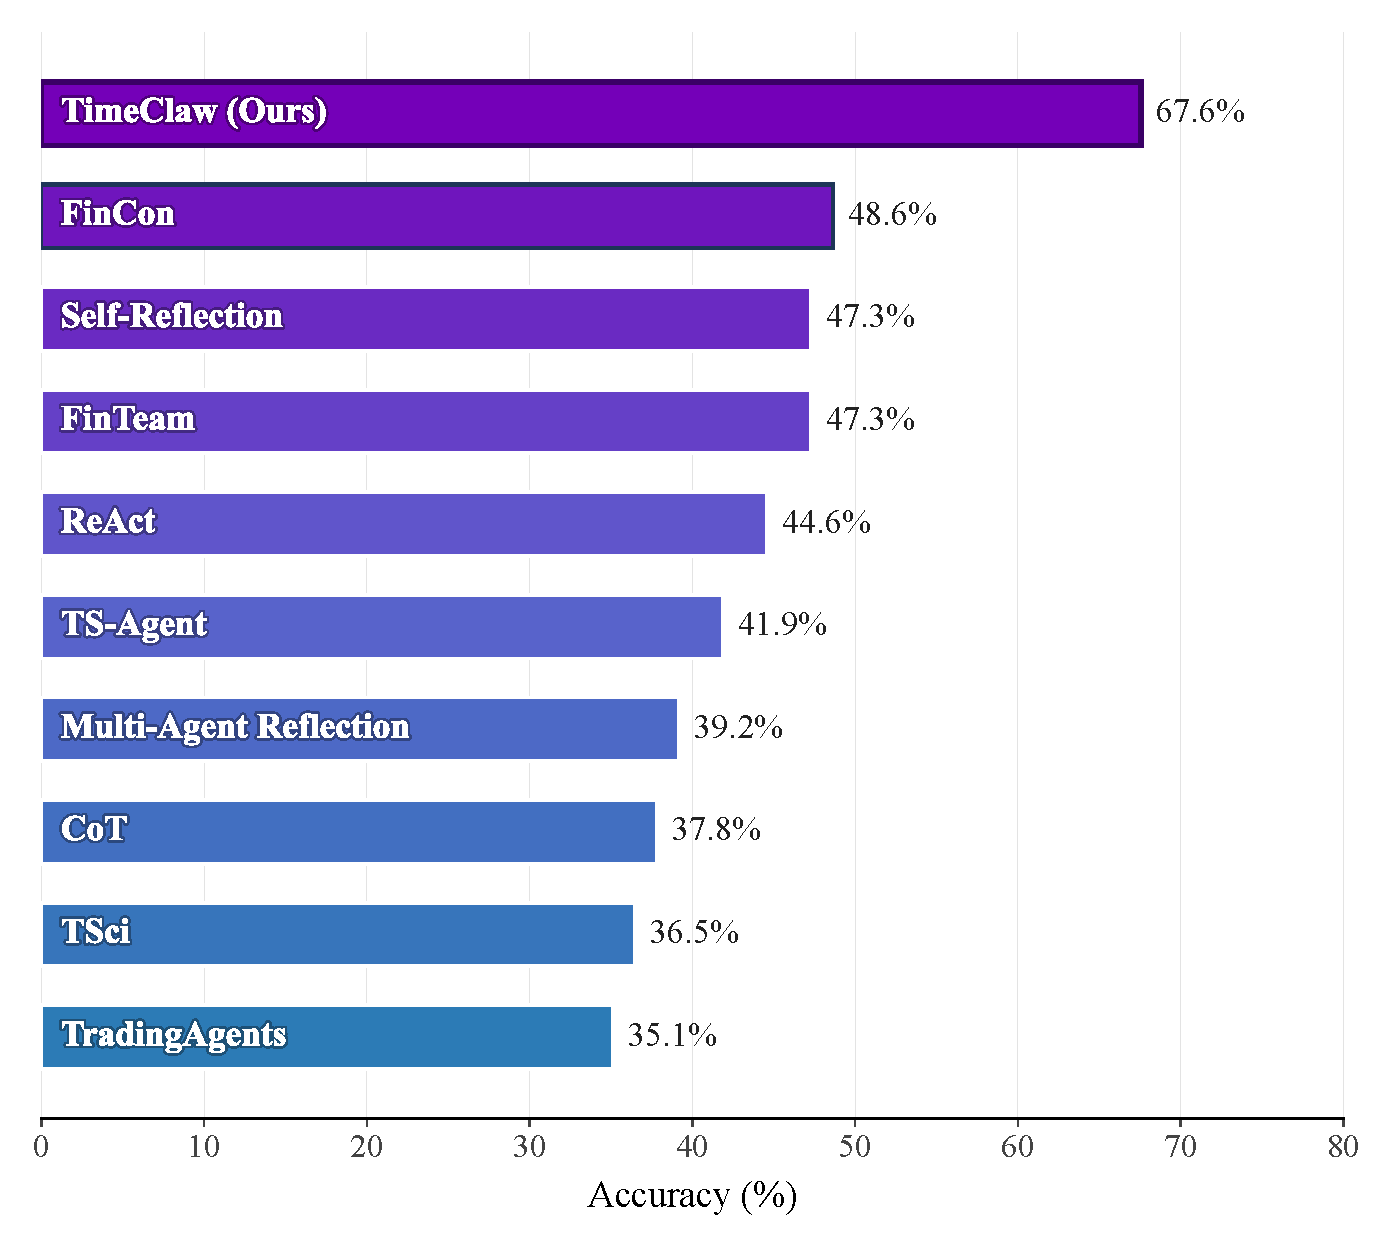
\includegraphics[width=\linewidth]{figures/tsaia_mc_accuracy_bar_purple.pdf}
\caption{
Performance on TSAIA. 
\method substantially outperforms both general agentic baselines and finance-specific agents, demonstrating its practical applicability in financial time-series analysis.
}
\label{fig:tsaia_mc_accuracy}
\end{figure}


We finally evaluate whether \method remains effective in a practical domain-specific setting. 
We use TSAIA~\citep{DBLP:journals/corr/abs-2509-01822}, a financial time-series analysis benchmark.
In addition to general agentic baselines, we include three finance-specific agent systems: FinCon~\citep{DBLP:conf/nips/YuYLDJCCSCLXZSX24}, FinTeam~\citep{DBLP:conf/nlpcc/WuWLYLZLCZW25}, and TradingAgents~\citep{DBLP:journals/corr/abs-2412-20138}. 

\noindent\textbf{Main Results.}
Figure~\ref{fig:tsaia_mc_accuracy} reports the multiple-choice accuracy on TSAIA. Notably, through the capability-evolution loop in Section~\ref{sec:evolve}, \method autonomously evolves three reusable routines from bank-building trajectories: \texttt{portfolio\_var}, \texttt{portfolio\_sharpe}, and \texttt{capm\_regression}. 
Equipped with these evolved routines, \method substantially outperforms all baselines by 38.9\% relative improvement. demonstrating that \method can acquire practical domain capabilities from experience.


\subsection{Ablation Study}

We conduct ablation studies to examine the effects of memory retrieval, backbone models, and framework components. 
As shown in Figure~\ref{fig:ablation_study}(a), enabling episodic memory retrieval improves both sMAPE and RCRPS, and larger retrieval sizes further improve performance. This shows that relevant past reasoning trajectories provide useful guidance for new contextualized time-series tasks.
Figure~\ref{fig:ablation_study}(b) shows that \method benefits from stronger LLM backbones, suggesting that time-series-native support complements general reasoning ability. 
Finally, Figure~\ref{fig:ablation_study}(c) shows that removing the tool harness, capability evolution, or memory all degrades performance, confirming that each part contributes to the final result. Due to page limitations, we provide further ablation studies in Appendix \ref{ap:full_experiments}, including memory bank size ablation and model family compatibility ablation.


\subsection{Case Study}

We provide detailed case studies in Appendix~\ref{ap:case_study} to illustrate how \method works on concrete tasks. 
These examples show how \method leverages textual context under identical numerical histories, uses retrieved memory to guide causal reasoning, and evolves reusable tools from prior trajectories. 
They qualitatively demonstrate that the gains of \method come from interpretable uses of context, memory, and experience-driven capability evolution.



\begin{figure*}[t]
  \begin{subfigure}[t]{0.32\linewidth}
    \centering
    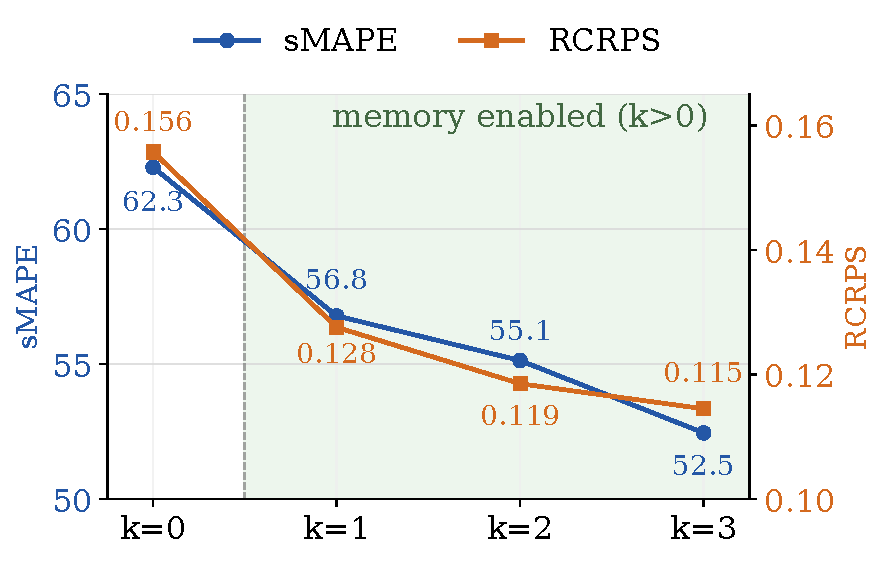
\includegraphics[width=\linewidth]{figures/hyperparameter/k_sensitivity.pdf}
    \caption{Retrieval Size Ablation.}
  \end{subfigure}\hfill
  \begin{subfigure}[t]{0.32\linewidth}
    \centering
    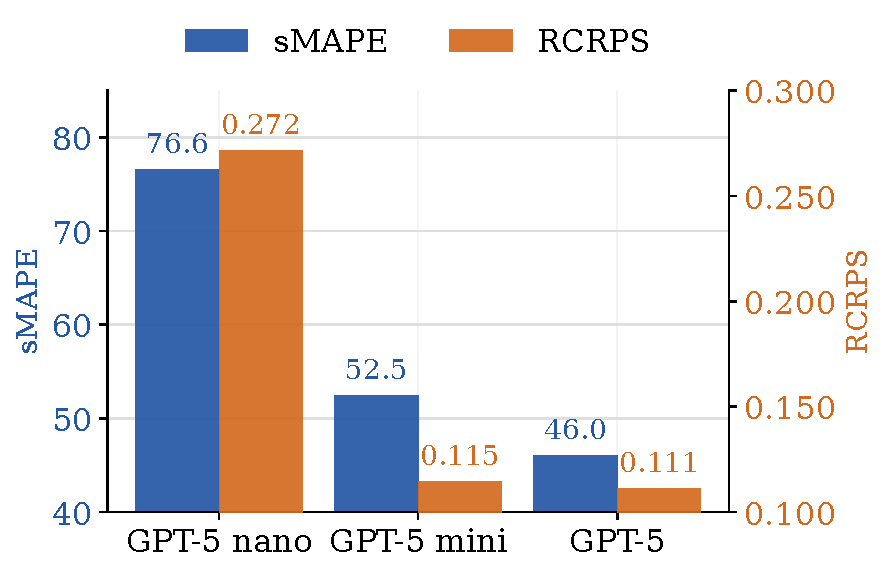
\includegraphics[width=\linewidth]{figures/hyperparameter/cik_model_ablation.pdf}
    \caption{Backbone Model Ablation.}
  \end{subfigure}\hfill
  \begin{subfigure}[t]{0.32\linewidth}
    \centering
    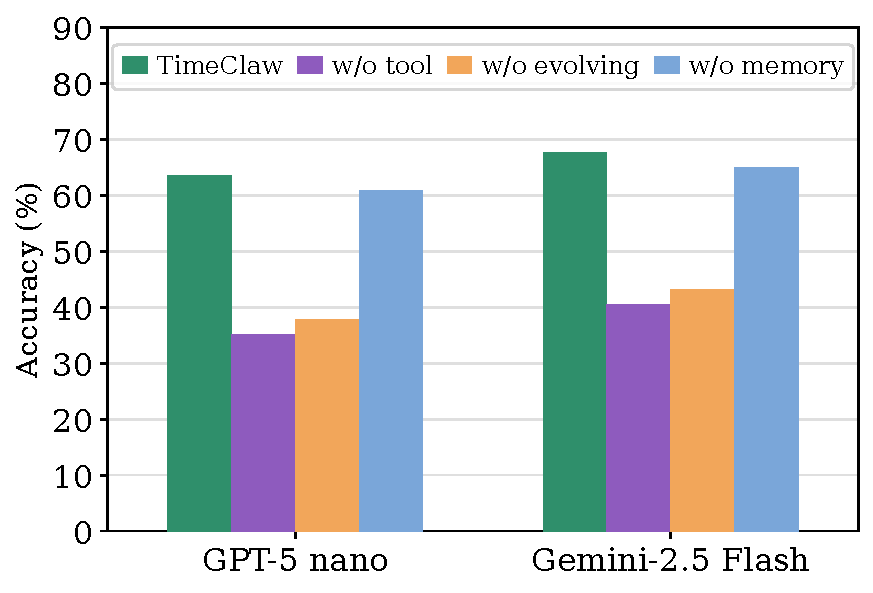
\includegraphics[width=\linewidth]{figures/hyperparameter/tsaia_ablation.pdf}
    \caption{Component Ablation.}
  \end{subfigure}\\[4pt]

\caption{
Ablation studies of \method. 
\textbf{(a)} Retrieval size ablation shows the benefit of enabling memory retrieval. 
\textbf{(b)} Backbone model ablation shows that \method consistently benefits from stronger LLM backbones. 
\textbf{(c)} Component ablation verifies the contributions of the tool harness, capability evolution, and memory. 
}
\label{fig:ablation_study}
\end{figure*}






